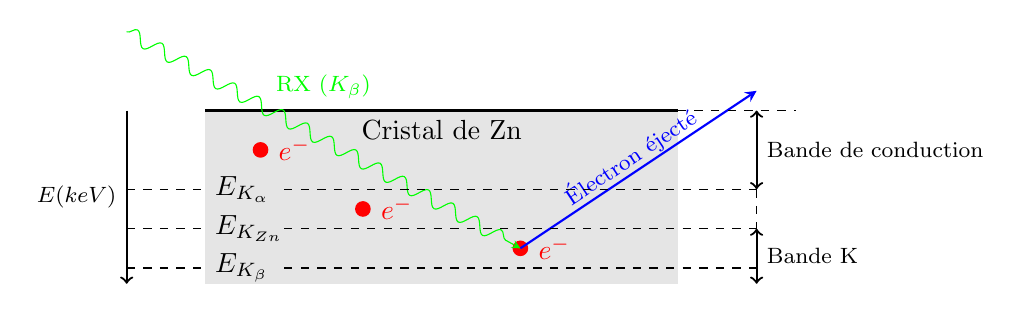
\begin{tikzpicture}[photon/.style={-stealth,decorate,decoration={snake,post length=1mm}}]
	
	% Dessiner le métal
	\fill[gray!20] (0,0) rectangle ++(6,-2.2);
	\draw[thick] (0,0) -- ++(6,0);
	\node[anchor=north] at (3,0) {Cristal de Zn};
	
	% Dessiner les électrons dans le métal
	\foreach \x/\y in {0.7/-0.5,2/-1.25,4/-1.75/-0.5}{
		\draw (\x,\y) node[circle,fill,inner sep=2pt, color=red,label={east:${\color{red}e^-}$}] {}; 
	}
	
	% Dessiner le photon incident
	\draw[photon,green] (-1,1) -- node[above=4mm,font=\footnotesize] {RX $(K_{\beta})$} ((4,-1.75);
	
	% Dessiner l'électron éjecté
	\draw[-stealth,blue,thick] (4,-1.75) -- node[above=-1mm,font=\footnotesize, sloped] {Électron éjecté} ++(3,2);
	
	
	\draw[<->, thick] (7,0) -- node[midway, right,font=\footnotesize] {Bande de conduction} (7,-1);
	
	\draw[dashed] (6,0) -- (7.5,0);
	
	\draw[dashed] (7,-1) -- (7,-1.5);
	
	\draw[<->, thick] (7,-1.5) -- node[midway, right,font=\footnotesize] {Bande K} (7,-2.2);
	
	\draw[->, thick] (-1,0) -- node[midway, left,font=\footnotesize] {$E(keV)$} (-1,-2.2);
	
	\foreach \y/\x  in {-1/$E_{K_{\alpha}}$, -1.5/$E_{K_{Zn}}$, -2/$E_{K_{\beta}}$} 
	{
		\draw [dashed] (-1,\y) -- (0,\y) node[right] {\x};
		\draw[dashed] (1,\y) -- (7,\y);
	}
	

	
\end{tikzpicture}


